\section{Introduction}

Integrating the utilization of program analysis (PA) tools early in the development process of modern, large-scale software systems is crucial in determining the weaknesses/vulnerabilities in the code. Consider, for instance, a scenario in which a developer wants to use an online question and answering (Q\&A) forum, e.g., StackOverflow (S/O), to learn how to use software libraries or frameworks. Typically, the answer to a posed question comes as a fragment/chunk of code, which later makes it to the production application, stemming from the copy-and-paste software reuse practice. Unfortunately, if the copied code fragment is vulnerable, i.e., possesses defects that one can potentially exploit, it will result in the application being prone to attacks. Verdi {\em et al.}~\cite{verdi-tse22} reviewed more than 72K C++ code snippets that migrated from 1,325 S/O answers, reporting a total of 99 vulnerable code snippets of 31 different types that made their way to 2,589 GitHub repositories.

Security researchers have proposed several automated approaches for vulnerability detection (VD) in software systems using program analysis (PA)~\cite{FlawFinder,RATS,viega2000its4,Checkmarx,HPFortify,Coverity}, as well as machine learning and deep learning (ML \& DL) \cite{fse21,chakraborty2020deep,zhou2019devign,li2018sysevr,li2018vuldeepecker} techniques. These approaches typically leverage program representations such as abstract syntax tree (AST), program dependence graph (PDG)~\cite{fse21,li2018vuldeepecker}, control-flow graph (CFG)~\cite{zhou2019devign}, data-flow graph (DFG)~\cite{zhou2019devign}, code property graph (CPG)~\cite{chakraborty2020deep}, etc., to model the vulnerable features. 
%However, extending such analyses to code snippets is not straightforward as they are often incomplete, unparseable, contain declaration/reference ambiguity, and may be interspersed between user comments. Currently, there exist tools such as PPA~\cite{ppa08}, which parse an incomplete code fragment to build the AST and extract data types in a best-effort manner, while StaType \cite{icse18} resolves the libraries and recovers only the fully-qualified names for references. However, the basic infrastructure for partial program analysis, i.e., for analyzing incomplete code is not yet available. 
%Such an infrastructure must include fundamental supports/services at the structural, semantic, and execution levels, thus enabling the static and dynamic analysis techniques to be built upon. 
%Let us refer to this as \textit{partial program analysis infrastructure}.
However, the PA tools employed to derive these program representations warrant the code to exist as complete program units, at the very least, at the method-level granularity. As a result, it is impossible to utilize such VD tools to find vulnerabilities in code snippets. A possible alternative would be to plug the code snippet into the method, resolve any ambiguities, and test it with a VD tool. However, such a strategy is limited. First, if a vulnerability is found, the efforts of integrating the code snippet into the existing method would be lost. Second, due to the black-box nature of DL models, we would not know the origin of the vulnerability, i.e., whether it arises due to the flawed code snippet or the existing part of the code.

Besides, analyzing code snippets is not straightforward as they are often incomplete, un-parseable, contain declaration/reference ambiguity, and are interspersed between user comments. Currently, there exist tools such as PPA~\cite{ppa08},~which parse an incomplete code fragment to build the AST and~ex\-tract data types in a best-effort manner, while StatType \cite{icse18} resolves the libraries and recovers only the fully-qualified names for references. However, deriving the program dependencies on incomplete code snippets is not yet possible. Let us call such an analysis, {\em partial program dependence analysis}.

In addition to vulnerability detection, such partial program dependence analysis is also beneficial to the other software engineering (SE) tasks that can tolerate a low level of errors and imprecision in building the dependencies. For example, consider code completion~\cite{codefill-icse22,facebook-icse21}, in which a model provides suggestions to complete partial code. Existing ML/DL-based code completion models are just based on the code sequences or utilize the syntactic structure in ASTs, but none leverage the program dependencies due to the nature of partial code. Next, consider the task of analyzing the code fragments in a bug report to connect it to the relevant source files for bug localization purposes~\cite{euler-fse19,icpc17}. Here too, a need for partial program dependence analysis can be observed.

In this work, we introduce \tool, a neural network-based tool to build
program dependence graph (PDG) for both complete and partial
programs. 

\begin{figure*}[hbt!]
\begin{center}
    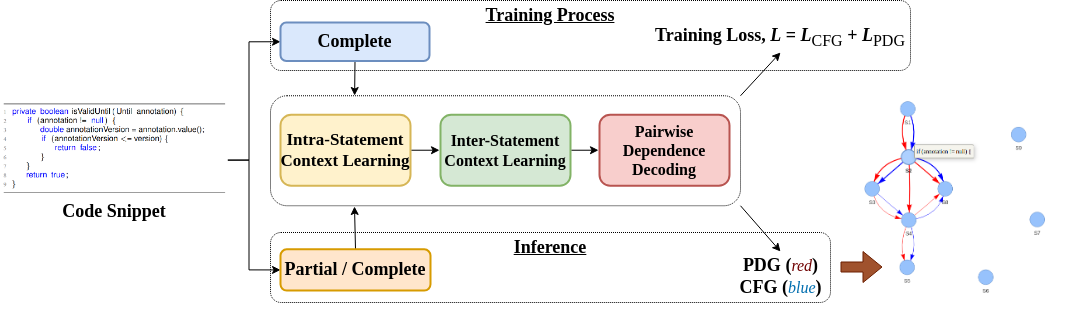
\includegraphics[width=\textwidth]{icse23-demo-figures/demo-arch3.png}
    \caption{\tool training and inference pipeline to enable dependence analysis for both partial and complete code.}
    \label{fig:model}
    \vspace{-8pt}
\end{center}
\end{figure*}

We draw motivation for such a data-driven, learning-based approach
from the following. First, ultra-large-scale software repositories,
e.g., GitHub (7M+ projects) and SourceForge (700k+ projects), contain
an enormous collection of programs. These repositories amount to 1B+
lines of code, 10M+ revision logs, and 3M+ issue reports. This wealth
of knowledge is an excellent source for {\tool}. Hindle {\em et
  al.}~\cite{naturalness-icse12} have shown that code has high
repetitiveness and predictability and can be captured well by
statistical models. Thus, we expect to build ML/DL models to learn
from those repositories.
%Second, Nguyen {\em et al.}~\cite{icse15} reported a high
%repetitiveness level for the sub-graphs in PDGs in open-source
%projects. Thus, {\tool} could learn the dependency structures
%extracted for whole programs in the existing code repositories and
%infer data types and program dependencies for partial programs. Third,
Second, in an empirical study on the repetitiveness, containment, and
composability of PDGs in open-source projects, Nguyen {\em et
  al.}~\cite{msr16} reported that among 17.5M PDGs with 1.6B PDG
subgraphs, 14.3\% of the PDGs have all of their subgraphs repeated
across different projects. Furthermore, in 15.6\% of the PDGs, at
least 90\% of their subgraphs are likely to have appeared before in
other projects.
%Second, Nguyen {\em et al.}~\cite{icse15} reported a high
%repetitiveness level for AST code structure in open-source
%projects. Thus, {\tool} infrastructure could help learn
%structure-level information from the ASTs extracted for whole programs
%in the existing code repositories and infer data types, partial ASTs
%for partial programs. Third, in an empirical study on the
%repetitiveness, containment, and composability of PDGs in open-source
%projects, the PI group~\cite{msr16} reported that among 17.5M PDGs
%with 1.6B PDG subgraphs, 14.3\% of the PDGs have all of their
%subgraphs repeated across different projects. Furthermore, in 15.6\%
%of the PDGs, at least 90\% of their subgraphs are likely to have
%appeared before in other projects.
%Thus, {\tool} could learn from PDGs with complete program dependencies retrieved from existing code repositories and derive the dependencies for the (partial) code fragment under study. The PI group also reported a high repetitiveness level for AST code structure in open-source projects~\cite{icse15}.
Thus, {\tool} could learn semantic-level information from the PDGs
with complete program dependencies retrieved from existing code
repositories and infer such dependencies for the partial code.


We design {\tool} to efficiently incorporate intra-statement and
inter-statement contextual features into statement representations,
thereby modeling program dependencies as a statement-pair dependence
decoding task. The key philosophy that drives our work is that the
dependency analyses of partial code can be learned from the analysis
of entire programs in the wealth of information obtained from
ultra-large-scale, open-source software repositories.


%Our key contributions are as follows:
%\begin{enumerate}
%    \item enable construction of interactive control-flow and program dependence graphs for \underline{partial} code snippets.
%    \item provide support to both Java and C++.
%    \item observe $\sim380\times$ markup against Joern PA tool.
%\end{enumerate}
